\graphicspath{{e02-04_ET-Grundlagen/}}

\chapter{Spannung, Strom, Widerstand und Leistung (E02--E04)}

% FIXME Figure wieder oben richtig einbauen
% \begin{wrapfigure}[0]{r}[-1cm]{0.5cm}
%  \vspace{-7cm}
%   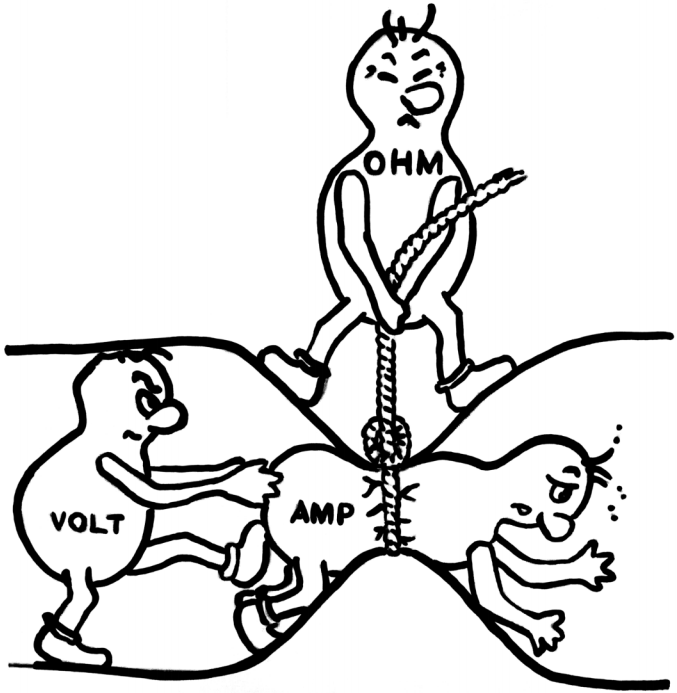
\includegraphics[scale=0.15]{e02-04_ET-Grundlagen/URI.png}
%  \vspace{-6cm}
% \end{wrapfigure}

%%%%%%%%%%%%%%%%%%%%%%%%%%%%%%%%%%%%%%%%%%%%%%%%%%%%%%%%%%%%%%%%%%%%%%%%
%% Theorie

\section{Theorie- und Prüfungsfragen}

%\loesung{
%\begin{figure}[H]
%\centering
%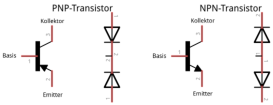
\includegraphics[scale=3]{Transistor/Bilder/PNP_NPN.pdf}
%\caption{1 und 2 - NPN- und PNP-Transistor}
%\end{figure}
%}

\mucho{1}{TB903}
{Welche Spannung lässt einen Strom von $2A$ durch einen Widerstand von
$50\Omega$ fließen?}%Frage
{$25V$}%A
{$200V$}%B
{$100V$}%C
{$52V$}%D
{C}%Lösung

\mucho{2}{TD302}
{Die Leerlaufspannung einer Gleichspannungsquelle beträgt $13,5V$. Wenn die
Spannungsquelle einen Strom von $1A$ abgibt, sinkt die Klemmenspannung auf
$12,4V$. Wie groß ist der Innenwiderstand der Spannungsquelle?}%Frage
{$1,1\Omega$}%A
{$1,2\Omega$}%B
{$12,4\Omega$}%C
{$13,5\Omega$}%D
{A}%Lösung

\mucho{3}{TB908}
{Ein mit einer künstlichen $50\Omega$-Antenne in Serie geschaltetes
HF-Amperemeter zeigt $2A$ an. Welche Leistung gibt der Sender ab?}%Frage
{$100W$}%A
{$200W$}%B
{$25\Omega$}%C
{$250\Omega$}%D
{B}%Lösung

\mucho{4}{TB104}
{Welche Gruppe von Materialien enthält nur Nichtleiter?}%Frage
{Pertinax, Polyvinylchlorid (PVC), Graphit}%A
{Epoxid, Polyethylen (PE), Polystyrol (PS)}%B
{Polyethylen (PE), Messing, Konstantan}%C
{Teflon, Pertinax, Bronze}%D
{B}%Lösung

\aufgabentext{
	\begin{enumerate}
	\item[5] \emph{\textbf{TC105-107}} Ordne den folgenden Schaltzeichen die Bezeichnungen LDR, PTC, NTC und VDR zu.\\
		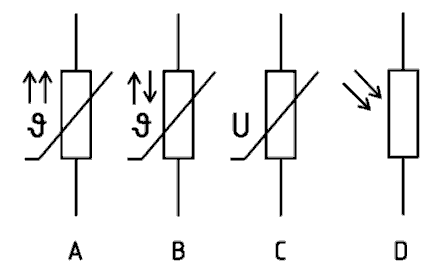
\includegraphics[scale=0.3]{Bild04.png}
		\loesung{Lösung: A PTC, B NTC, C VDR, D LDR}
		\end{enumerate}
	}

\mucho{6}{TC101}
{Die Farbringe gelb, violett und orange auf einem Widerstand mit 4 Farbringen bedeuten einen Widerstandswert von}%Frage
{$4,7k\Omega$}%A
{$47k\Omega$}%B
{$470k\Omega$}%C
{$4,7M\Omega$}%D
{gelb: 4; violett: 7; orange: $\cdot 10^3$; ergibt $47000\Omega$ oder $47k\Omega$: B}%Lösung

\mucho{7}{TC110}
{Welchen Wert hat ein SMD-Widerstand mit der Kennzeichnung 221?}%Frage
{$221\Omega$}%A
{$22k\Omega$}%B
{$22\Omega$}%C
{$220\Omega$}%D
{D}%Lösung

\mucho{8}{TC108}
{Ein Widerstand hat eine Toleranz von $10 \%$. Bei einem nominalen Widerstandswert von $5,6 k\Omega$ liegt der tatsächliche Wert zwischen}%Frage
{$4760$ und $6440 \Omega$}%A
{$5040$ und $6160 \Omega$}%B
{$4,7$ und $6,8 k\Omega$}%C
{$5,2$ und $6,3 k\Omega.$}%D
{B}%Lösung

\mucho{9}{TD108}
{Die Gesamtspannung U an folgendem Spannungsteiler beträgt $12,2V$. Die
Widerstände haben die Werte $R_1 = 10k\Omega$ und $R_2 = 2,2k\Omega$. Wie groß
ist die Teilspannung $U_2$?\\ 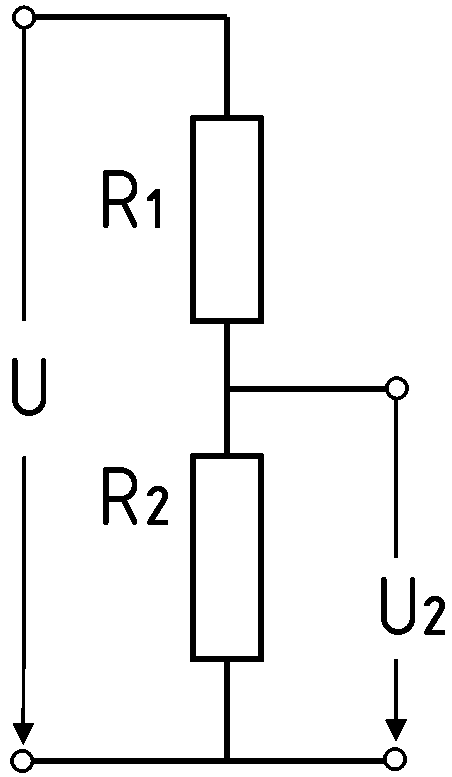
\includegraphics[scale=0.15]{Spannungsteiler.png}}%Frage
{$2,20V$}%A
{$2,64V$}%B
{$10,0V$}%C
{$1,22V$}%D
{A}%Lösung

\mucho{10}{TD103}
{Wie groß ist der Ersatzwiderstand der Gesamtschaltung? 
$R_1 = 500\Omega$, $R_2 = 500\Omega$ und $R_3 = 1k\Omega$\\ 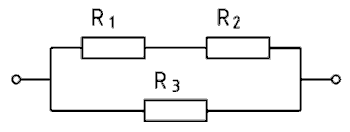
\includegraphics[scale=0.4]{Parallelschaltung.png}}%Frage
{$250\Omega$}%A
{$500\Omega$}%B
{$1k\Omega$}%C
{$2k\Omega$}%D
{B}%Lösung

%%%%%%%%%%%%%%%%%%%%%%%%%%%%%%%%%%%%%%%%%%%%%%%%%%%%%%%%%%%%%%%%%%%%%%%%
%% Praxis

\clearpage

\section{Grundlagen Breadboard/Messtechnik: U, I, R, P}

In diesem ersten Praxisteil Elektronik geht es darum euch mit dem Kursmaterial
vertraut zu machen und erste Schaltungen zu bauen und zu messen. Ablauf:

\begin{enumerate}
  \item Vorstellung des Kurskofferskonzepts und der Werkzeugtaschen
  \item Einführung Steckbrett
  \item Praxisaufgaben
\end{enumerate}

{
  \begin{wrapfigure}{r}{0.4\textwidth}
    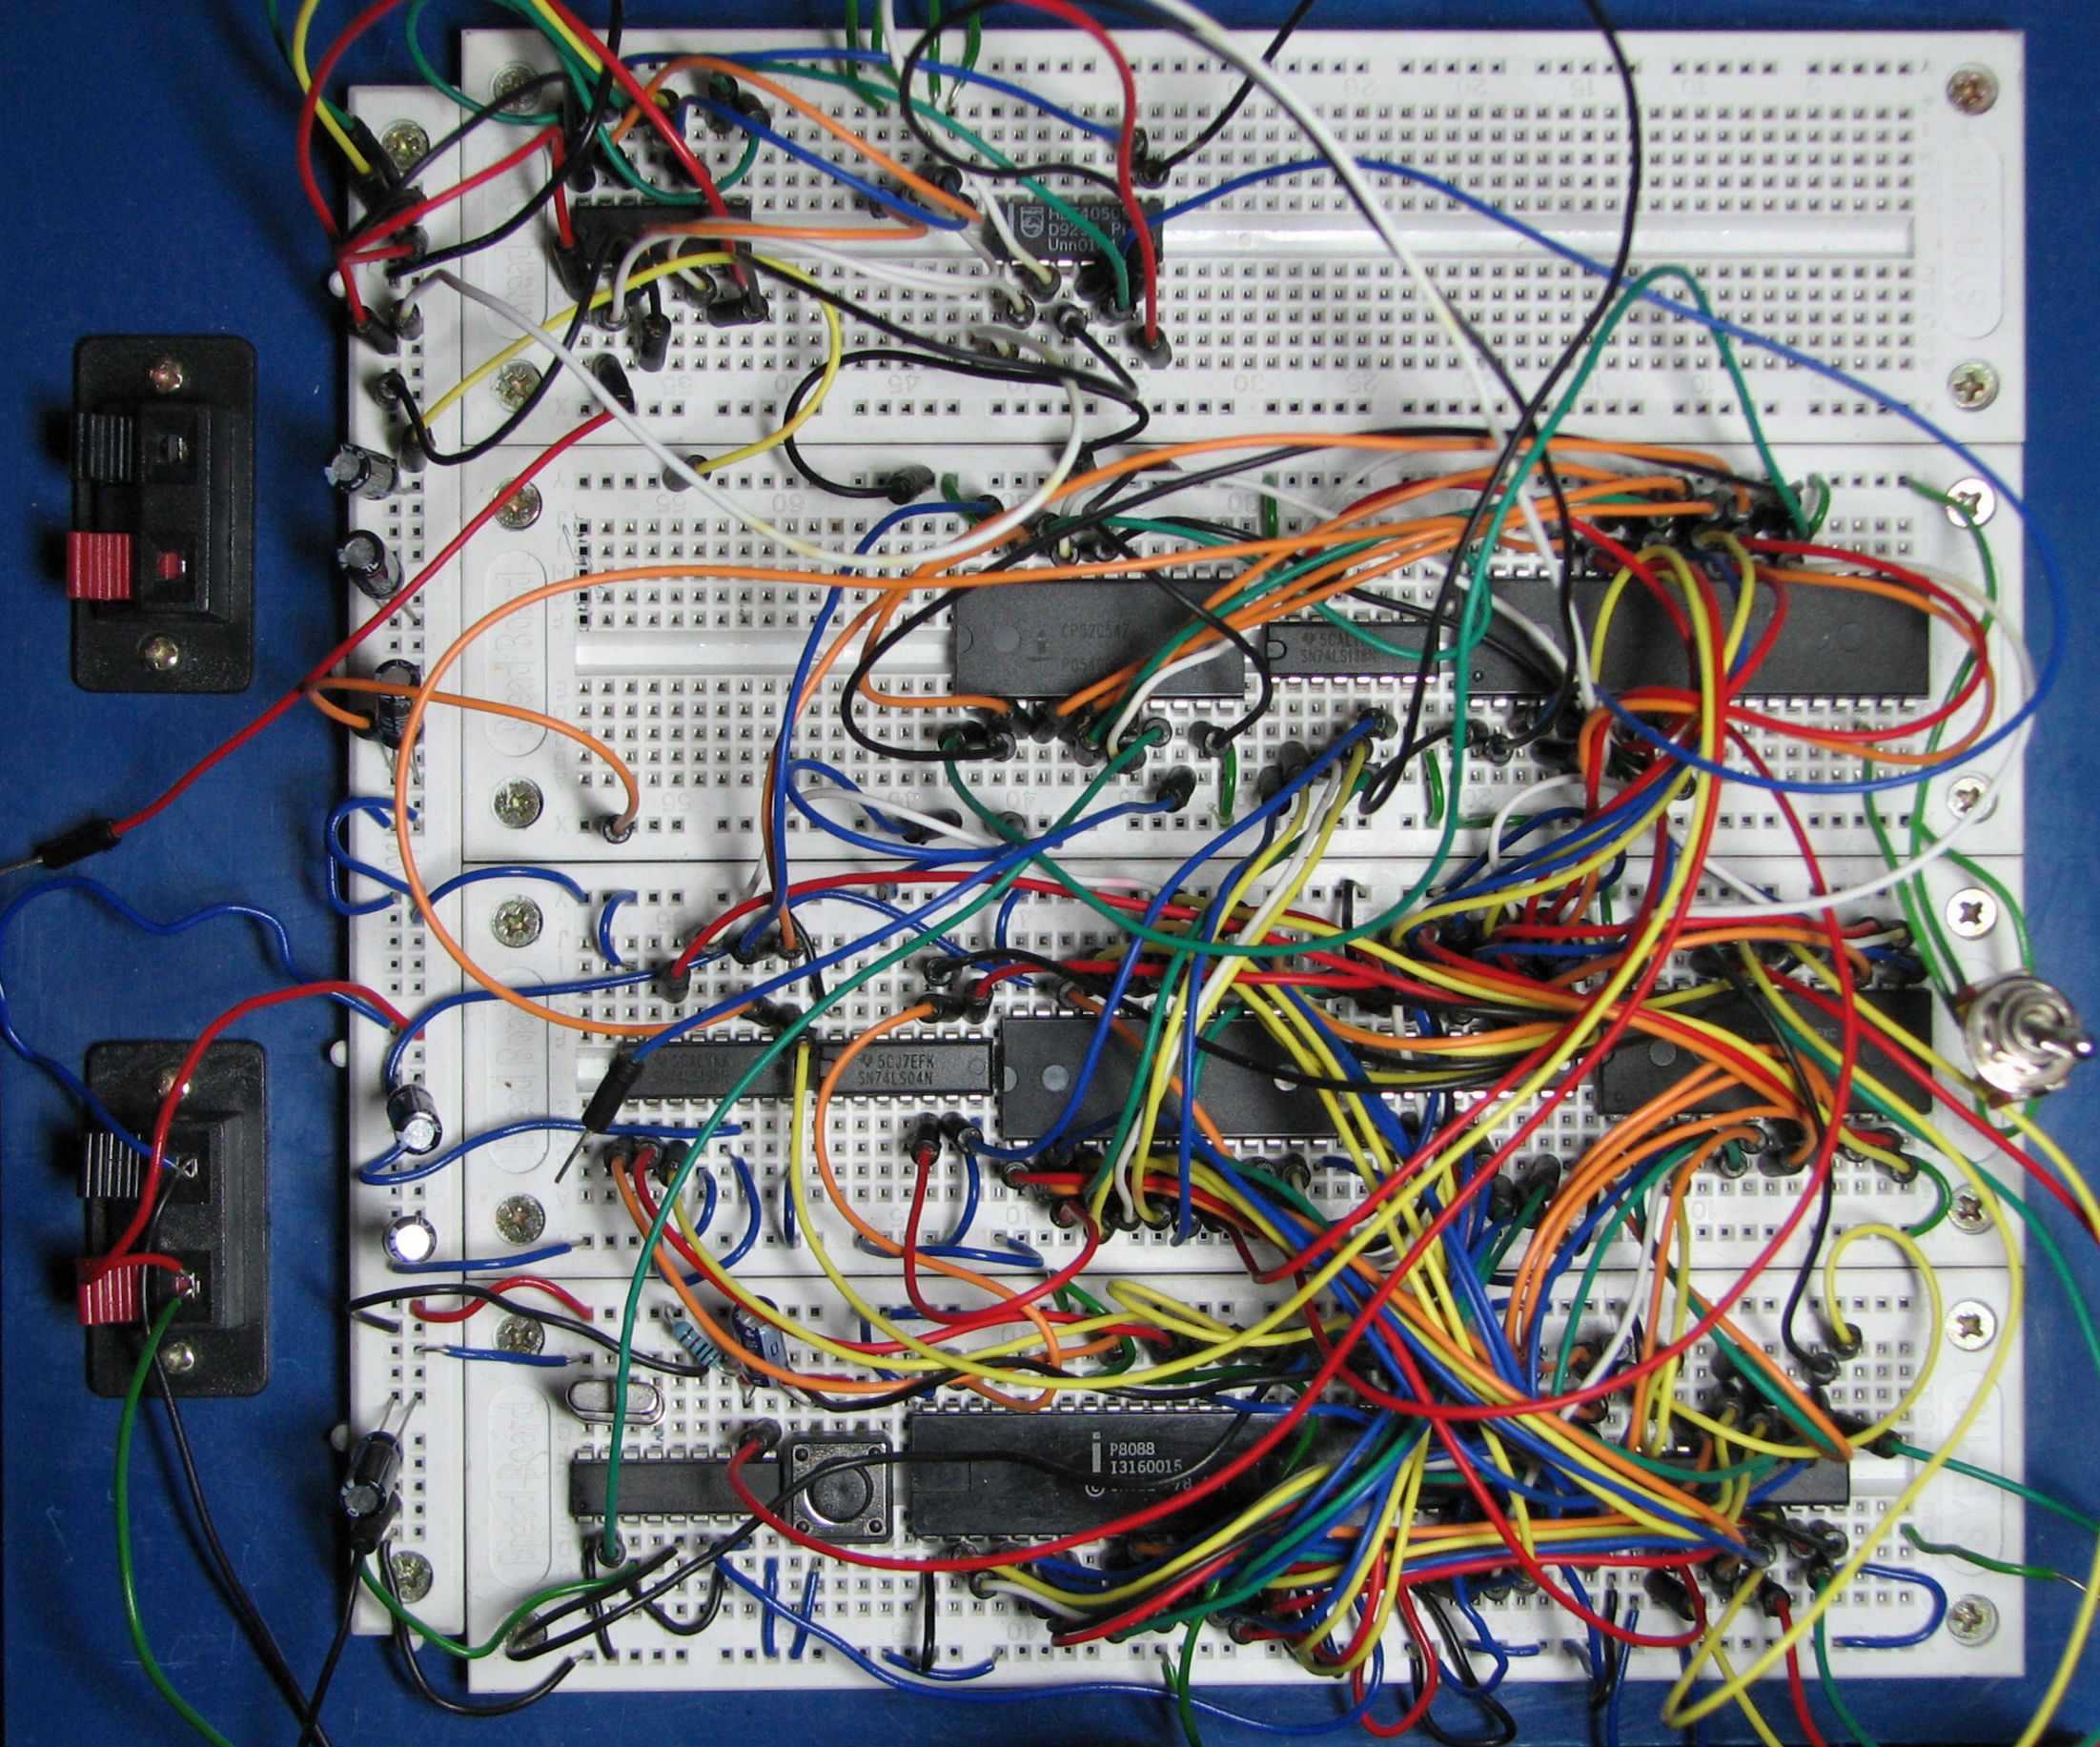
\includegraphics[width=0.38\textwidth]{Breadboard_complex.jpg}
  \end{wrapfigure}

  \paragraph{Vorbereitungsaufgabe}

  \emph{-- keine --}

  \loesung{Besondere Vorbereitungen: -- keine --}

  \paragraph{Material}

  \begin{itemize}
    \item Breadboard
    \item 9V-Blockbatterie oder 6--9V-Batteriefach
    \item Steckbrücken-/kabel
    \item LED
    \item 2x Widerstand (unbekannt) \loesung{470 $\Omega$ \& 1k $\Omega$}
  \end{itemize}
}

\paragraph{Hinweise}

Achtet darauf die Pole des Batteriepacks nicht kurzzuschließen -- wird sehr heiß
und blubbert!

\paragraph{How to Breadboard}

Ein Breadboard bzw. Steckbrett erlaubt schnelle Versuche mit THT-Bauteilen. Die
Benutzung ist in Abbildung \ref{fig:breadboard} dargestellt.

\begin{figure}[htbp]
  \centering
  \subfigure[Leeres Breadboard]{
    \label{fig:breadboard_leer}
    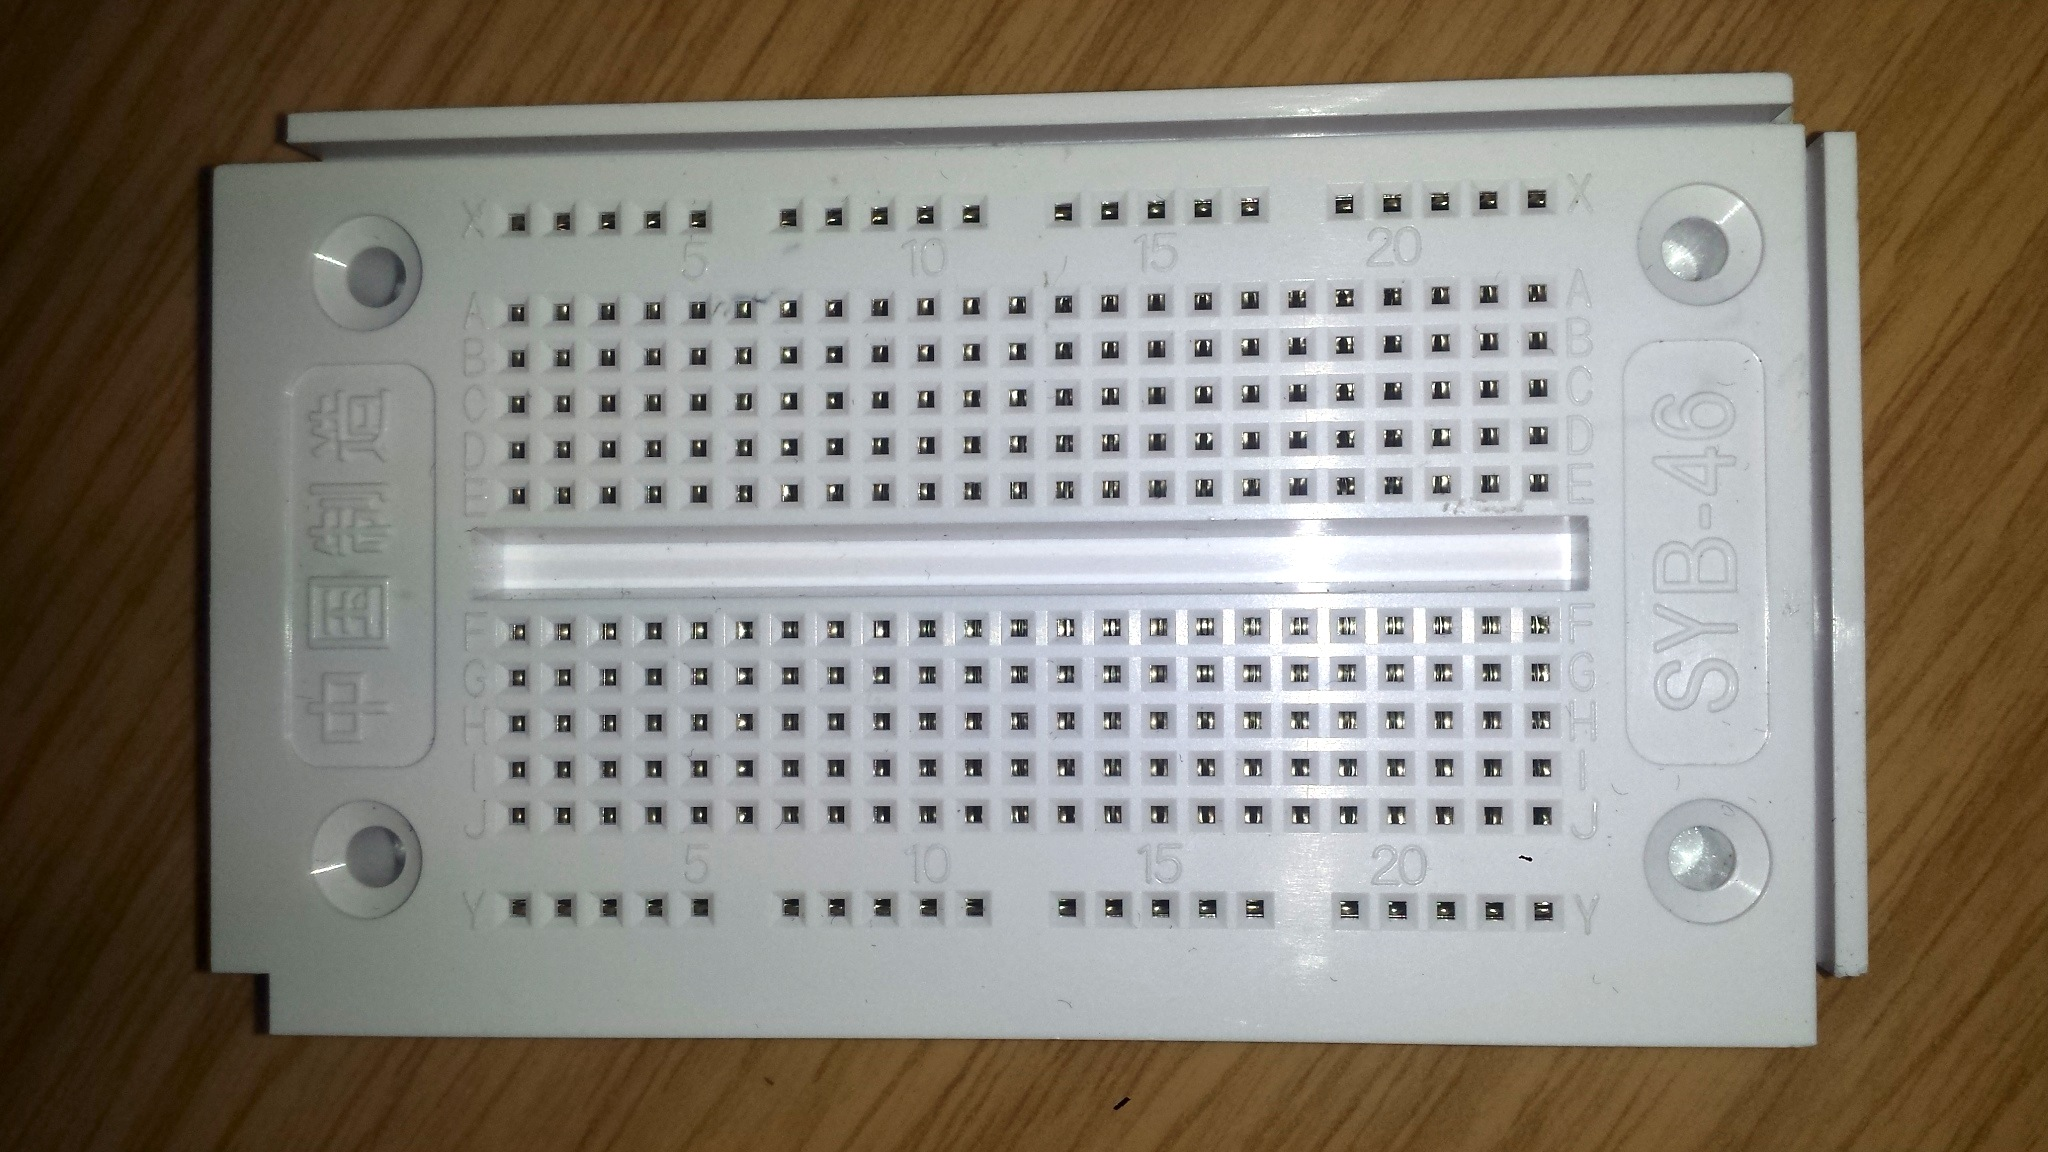
\includegraphics[width=0.3\textwidth]{Leeres_Board.jpg}
  }
  \subfigure[Bestückt mit Bauteilen]{
    \label{fig:breadboard_parts}
    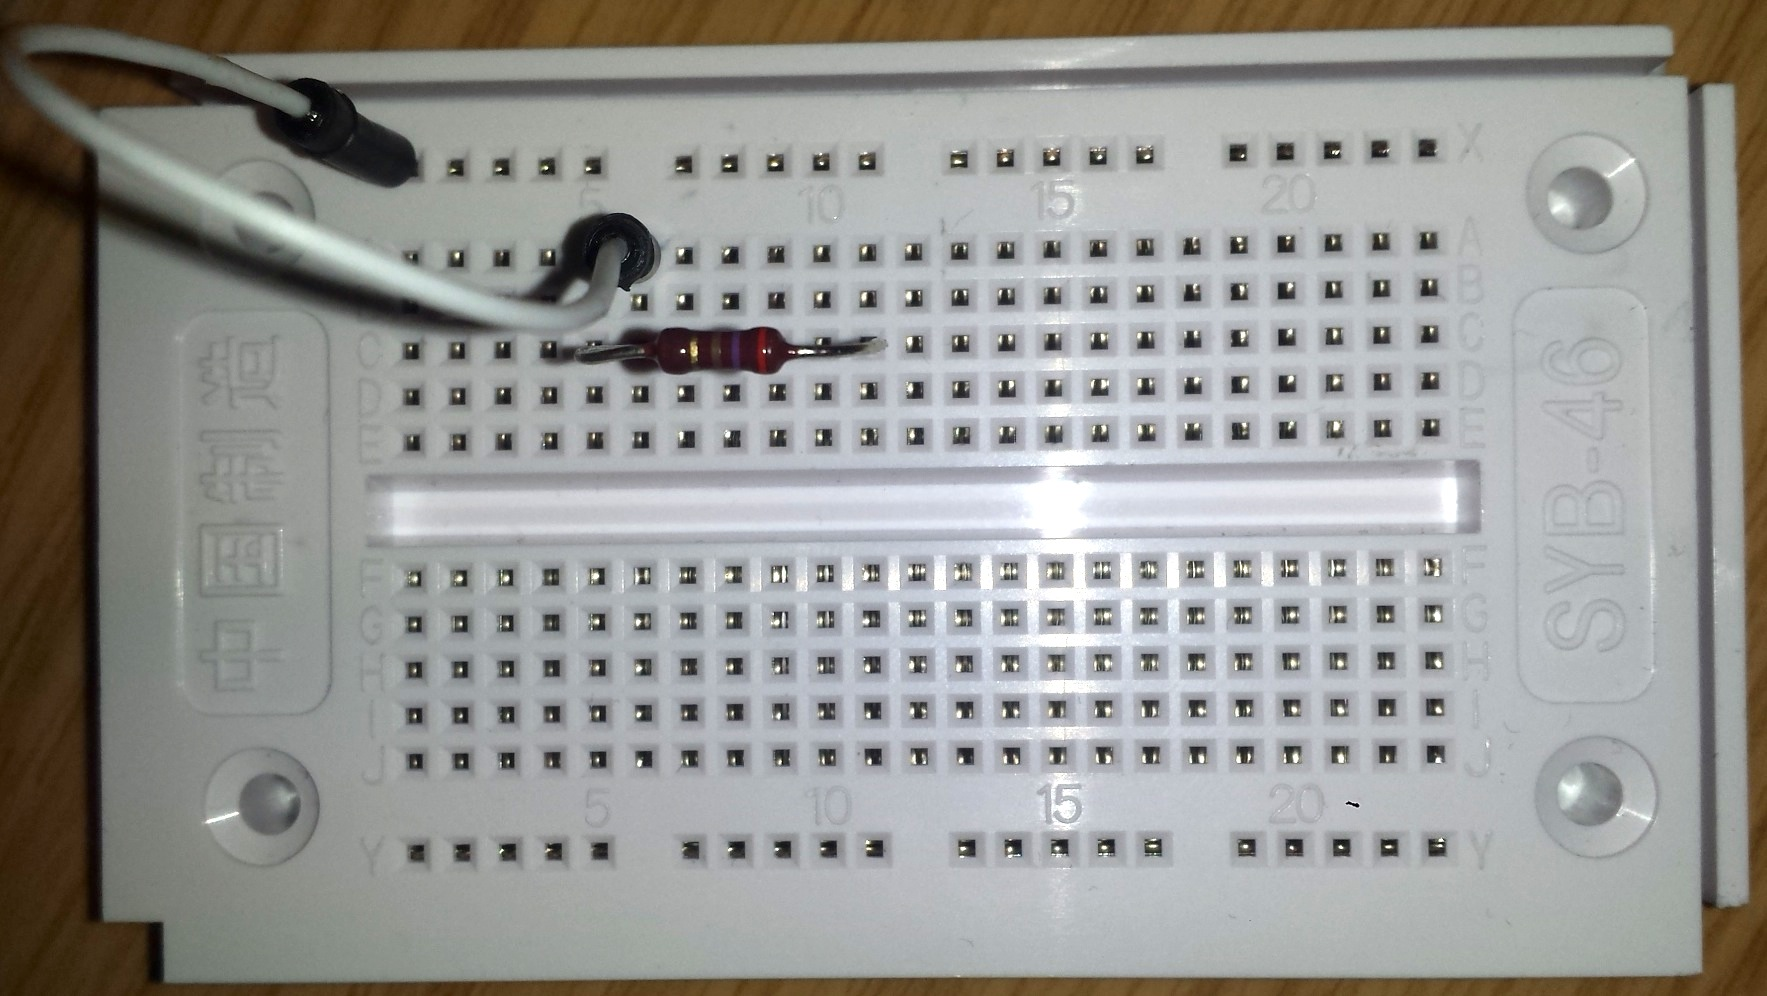
\includegraphics[width=0.3\textwidth]{Wiederstand_eingebaut.jpg}·
  }
  \subfigure[Verbindungen im Breadboard]{
    \label{fig:breadboard_lanes}
    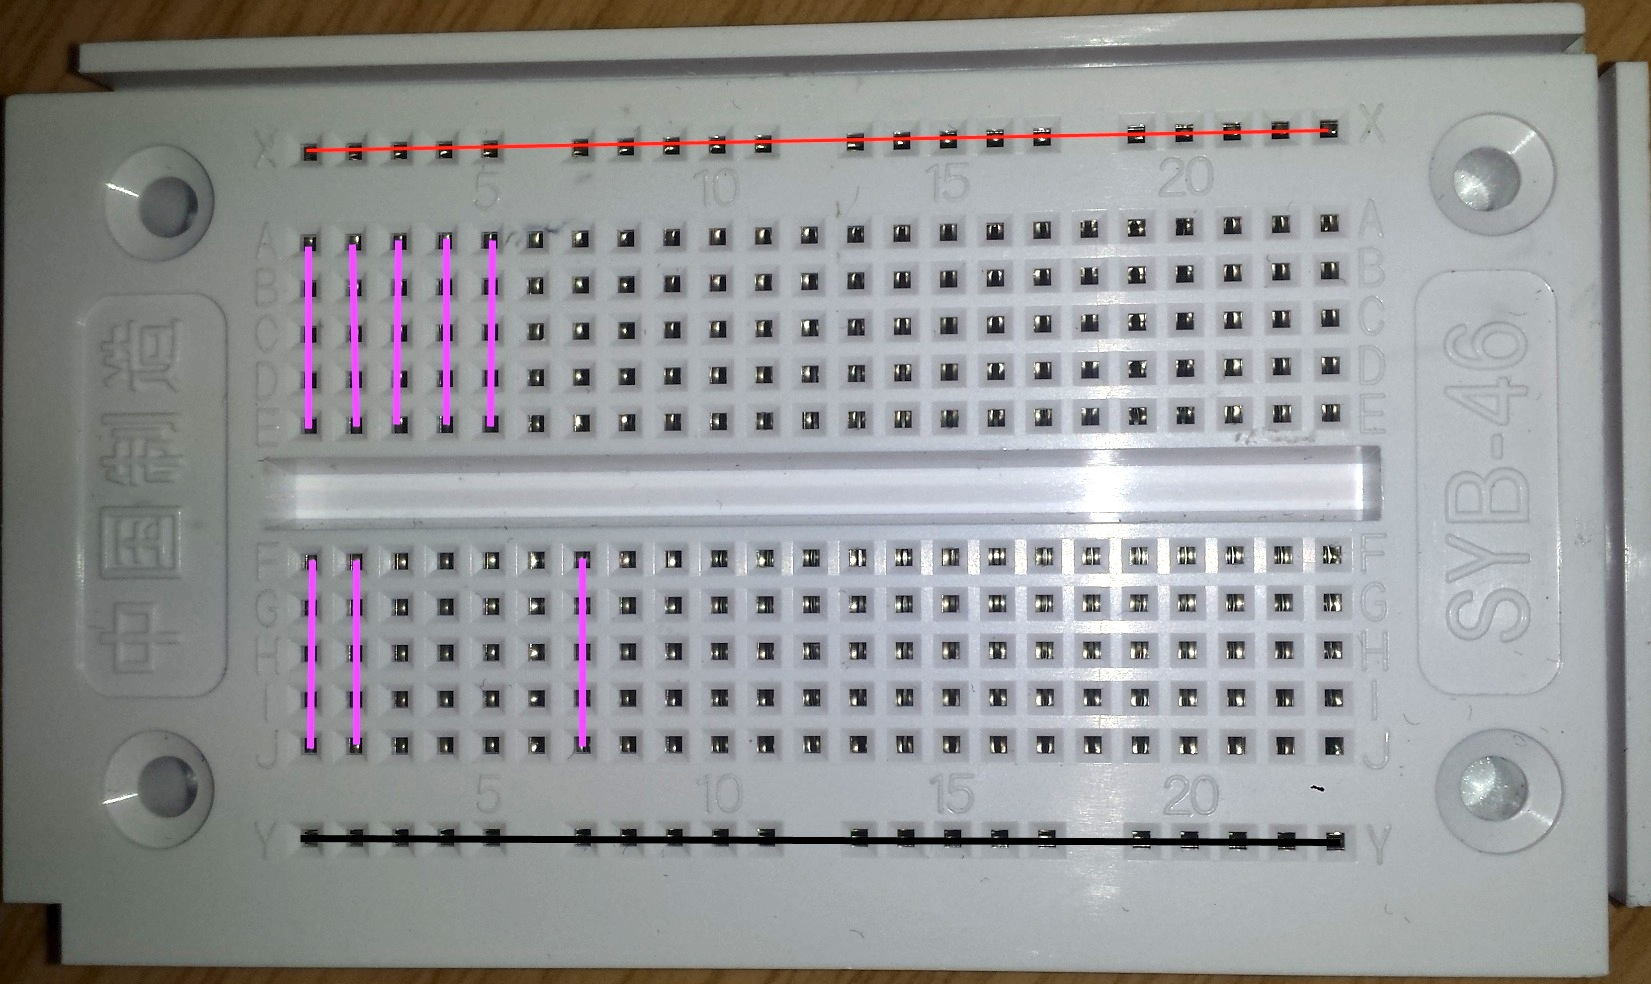
\includegraphics[width=0.5\textwidth]{Leeres_Board_verbindungen.jpg}
  }
  \caption{Mini-Breadboard SYB-46 \cite{afutub}} % FIXME citation
  \label{fig:breadboard}
\end{figure}

% TODO e99/Steckbrett_ersteUebung.png selber/gemeinsam stecken oder weglassen?

\clearpage

\paragraph{Aufgaben}

% DONE Schaltpläne einfügen? Nein, das muss so gehen.

\begin{enumerate}
  \item Wie ist ein übliches Batteriefach aufgebaut und wie verhalten sich dort
    Spannung und Strom? \\
    \loesung{Spannungen der Zellen addieren sich in Reihe, Strom überall
    gleich -- analog dazu: auch eine Batterie selbst ist meist eine gestapelte Zelle}
  \item Ihr habt zwei Widerstände zur Verfügung. Bestimmt die Bauteilwerte
    anhand der Ringe (vgl. Formelsammlungen im Anhang \ref{att:formela},
    \ref{att:formele} und \ref{att:formel+}) und messt sie nach.
    \begin{center}
    R1 = \dots \loesung{470} $\Omega$ \\
    R2 = \dots \loesung{1k} $\Omega$ \\
    Toleranz: 5\%
    \end{center}
  \item Baut einen Stromkreis mit einer LED und den beiden Vorwiderständen
    (einmal seriell, einmal parallel) auf dem Breadboard auf. Was ändert sich?
    Berechnet und messt jeweils den Gesamtvorwiderstand! \\
    \loesung{Parallel: 213 $\Omega$, Serie 1470 $\Omega$}
  \item Verwendet die parallele Gesamtschaltung für die weiteren Messungen
    \begin{enumerate}
      \item Messt die Einzelströme durch die Widerstände! Rechnet nach! \\
        \loesung{Messung: 470 $\Omega$: $\approx$ 20-30mA, 1k $\Omega$: $\approx$ 10 mA, $U_r$ = 6,6 V, $I_{ges}$ = 30 mA}\\
        \loesung{Rechnung: 470 $\Omega$: $\approx$ 14 mA, 1k $\Omega$: $\approx$ 6,6 mA, $I_{ges}$ = 20,6 mA}
      \item Messt die notwendigen Spannungen um die Leistungsaufnahme der
        Gesamtschaltung sowie der LED zu berechnen! Was fällt euch auf? \\
        \loesung{$I_{ges}$ = 30 mA, $U_{ges}$ = 9,11 V, $U_{LED}$ = 2,45 V, $P_{LED}$ = 73 mW, $P_{ges}$ = 273 mW, $\eta$ = 27\%}
    \end{enumerate}
  \item Zusatzaufgabe: Spannungsteiler LED\\ % FIXME siehe "Zusatzaufgabe" unten

\end{enumerate}

%%%%%%%%%%%%%%%%%%%%%%%%%%%%%%%%%%%%%%%%%%%%%%%%%%%%%%%%%%%%%%%%%%%%%%%%
%% Archiv: Aufgaben von DC4LW aus den alten Folien e04

%\subsection*{Übung 1}
%\begin{frame}
%  \begin{columns}
%    \column{0.4\textwidth}
%    \begin{center}
%      \begin{figure}
%        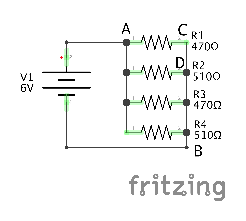
\includegraphics[width=1\textwidth]{e04/Uebung1_Schaltplan.pdf}
%      \end{figure}
%    \end{center}
%    \column{0.55\textwidth}
%    \begin{alertblock}{Aufgabe 1}
%      Baue die Schaltung auf dem Steckbrett auf.\\
%      Berechne den Ersatzwiderstand. Miss zur Überprüfung den Gesamtwiderstand.
%    \end{alertblock}
%    \begin{alertblock}{Aufgabe 2}
%      Berechne die Spannung über $R_1$, $R_2$, $R_3$ und $R_4$. Miss zur Überprüfung nach.\\
%      Miss und erkläre die Spannungen über $A$---$B$, $A$---$C$ und $A$---$D$.
%    \end{alertblock}
%  \end{columns}
%  \begin{alertblock}{Aufgabe 3}
%    Berechne die Ströme durch $R_1$, $R_2$, $R_3$, $R_4$ und den Gesamtstrom. Miss zur %Überprüfung nach.
%  \end{alertblock}
%\end{frame}

%\subsection*{Übung 2}
%\begin{frame}
%  \begin{columns}
%    \column{0.4\textwidth}
%    \begin{center}
%      \begin{figure}
%        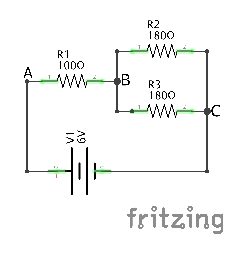
\includegraphics[width=1\textwidth]{e04/Uebung2_Schaltplan.pdf}
%      \end{figure}
%    \end{center}
%    \column{0.55\textwidth}
%    \begin{alertblock}{Aufgabe 1}
%      Baue die Schaltung auf dem Steckbrett auf.
%      Berechne den Ersatzwiderstand. Miss zur Überprüfung den Gesamtwiderstand.
%    \end{alertblock}
%    \begin{alertblock}{Aufgabe 2}
%      Berechne die Spannung über $R_1$, $R_2$ und $R_3$. Miss zur Überprüfung nach.\\
%      Miss und erkläre die Spannungen über $A$---$B$, $A$---$C$ und $B$---$C$.
%    \end{alertblock}
%  \end{columns}
%  \begin{alertblock}{Aufgabe 3}
%    Berechne die Ströme durch $R_1$, $R_2$, $R_3$ und den Gesamtstrom. Miss zur Überprüfung %nach.
%  \end{alertblock}
%\end{frame}

%\subsection*{Übung 3}
%\begin{frame}
%  \begin{alertblock}{Zusatzaufgabe}
%    Die rote Leuchtdiode benötigt einen Strom von $20mA$. Für die Aufgabe sei erstmal angenommen, dass keine Spannung über die Leuchtdiode abfällt. Dimensioniere einen Spannungsteiler so, dass mit der gegebenen Batterie von 6V an der Leuchtdiode eine Spannung von 3V bis 5V anliegt. Gegeben sind die Widerstände in der Größe $4\times100\Omega$, $2\times180\Omega$, $4\times470\Omega$ und $2\times510\Omega$. Berechne zuerst den Spannungsteiler und zeichne einen Schaltplan.
%  \end{alertblock}
%%  \begin{alertblock}{Aufgabe 2}
%%    Baue die Schaltung auf. Die abgeflachte Seite der Leuchtdiode zeigt zu Minus. Miss den %Strom durch die Leuchtdiode. Miss die Spannung über die Widerstände. Wie lautet die %Gesamtsumme der Spannungen über die Widerstände? Erkläre.
%%  \end{alertblock}
%%  \begin{alertblock}{Aufgabe 3}
%%    Die Leuchtdiode soll dunkler leuchten. Muss dazu mehr oder weniger Strom fließen? Wie %sind die Widerstände zu dimensionieren?
%%  \end{alertblock}
%\end{frame}
